Nesta prática busca-se comparar os resultados de aprendizado supervisionado realizado nos experimentos anteriores com o método Label Propagation.

\subsection{Descritor LBP}
\subsubsection{Seleção dos parâmetros para o método Label Propagation}
O método Label Propagation pode ser utilizado com o kernel de k vizinhos mais próximos (K-Nearest Neighbors - KNN) e funçao de base radial (Radial Basis Function - RBF). Para o  primeiro caso deve-se definir o número máximo de iterações o número de vizinhos e outros. Para o RBF deve-se definir o valor gamma, a quantidade máxima de iterações e outros.

Para este experimento variou-se o kernel entre KNN e RBF, o valor gama em 20, 25, 30, a quantidade máxima de iterações em 300, 500, 1000 e o número de vizinhos em 7, 14, 21 e 28. Para cada combinação foi feita a validação cruzada em 5 partições. O critério para definição dos melhores parâmetros foi a média da acurácia. Os melhores parâmetros para o kernel KNN e RBF estão descritos na Tabela~\ref{tab:meida_acuracia_lp_lbp}. Para todos os classificadores o desempenho da acurácia apresentou queda quando comparado as técnincas supervisionadas. Contudo existe a redução de 600 imagens rotuladas para 360. A comparação com os resultados das práticas supervisionadas podem ser vistas na Figura~\ref{fig:super_vs_semi_lbp}.


\begin{table}[!htbp]
    \caption{Média e desvio padrão para acurácia}
    \begin{center}
        \begin{tabular}{lllllll}
        	Kernel & Iteração & Vizinhos & Gamma &  Média & Desv. Pad. & Pos. \\
        	\hline
        	KNN    & 300             & 7                  & n/a  & 0.39       & 0.021               & 1       \\
        	\hline
        	RBF    & 300             & n/a                & 20   & 0.10       & 0.003               & 13      \\
        \end{tabular}
    \label{tab:meida_acuracia_lp_lbp}
    \end{center}
\end{table}

\begin{figure}[!htbp]
	\centering
	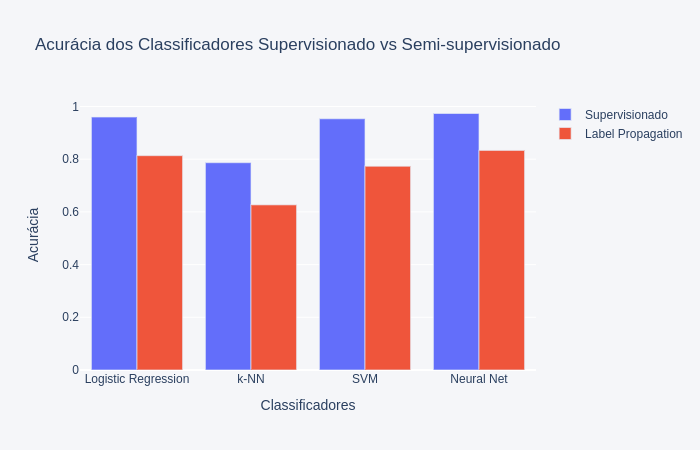
\includegraphics[width=1.0\linewidth,clip=true,trim=0cm 0cm 0cm 0cm, keepaspectratio=true]{bar_supervisionado_vs_semi_lbp.png}
	\caption{Supervisionado vs Semi-supervisionado.}
	\label{fig:super_vs_semi_lbp}
\end{figure}
